\chapter{Methodology}\label{chap:chap4}

\section*{}



\section{Introduction}

According to the state of the art presented in chapter two, there are many means to, in some kind of automatic way, improve an applications performance. During my research, my focus was to find ways to automatically enhance the execution time in applications and programs. For this propose, Kremlin had a crucial impact in other to understand the viability of automatically parallelise code.

To study the utility and impact of automatic tools, the matrix multiplication algorithm will be used as a reference to make the performance comparison between original algorithm, an expert manually parallelising the original algorithm and using the Kremlin's indication to parallelise the original algorithm.

To increase the credibility of this experiment, two similar algorithms for the matrix multiplication were used. As mentioned and explained in the chapter two, there is the traditional way of multiplying square matrices, naming as a quick reference \textit{Mult} algorithm, see in the appendix's list ~\ref{code:onmul} this algorithm implementation, written in C++ programming language; and the optimized algorithm that multiplies each element from the first matrix with the correspondent line of this matrix element but for the second matrix, naming this algorithm as \textit{MultLine}, see in the appendix's list ~\ref{code:onmuline} this algorithm implementation, written in C++ programming language. These algorithms differs from one another in the variables preparation and the order of the loops, which differs in the memory access. The \textit{MultLine} algorithm is an optimized version for matrix multiplication because it takes advantages of what is preloaded in cache and starts pre-calculating the intermediate values that will lead to the final and correct result of the multiplication, which means that the computer won't need to load unnecessary values to cache memory and/or will need afterwards.  

Several experiments were conducted to understand the influence of Kremlin's indications versus code being manually parallelized  by an expert. The data's length, in this case, the matrix size; the number of threads used and if the code was parallelized were the used metrics to evaluate the results, based on a comparison of the execution time, changing these variables.

In this chapter it is explained the methodology and the steps followed that guided to report in the Results and Discussion chapter the results and conclusions obtained from the obtained outcomes coming from de experiences. This chapter also includes  detailed information of the acquired data from the conducted experiences, as in, how it is obtained and its meaning; also includes the methods that were used to analyse the obtained data and the reason behind those methods; how the data was validated in order to verify its correctness, accuracy and reliability; and, in the end, it includes the setup and material used to conduct such experiments.



\section{Research Method}

\begin{figure}[t]
	\begin{center}
		\leavevmode
		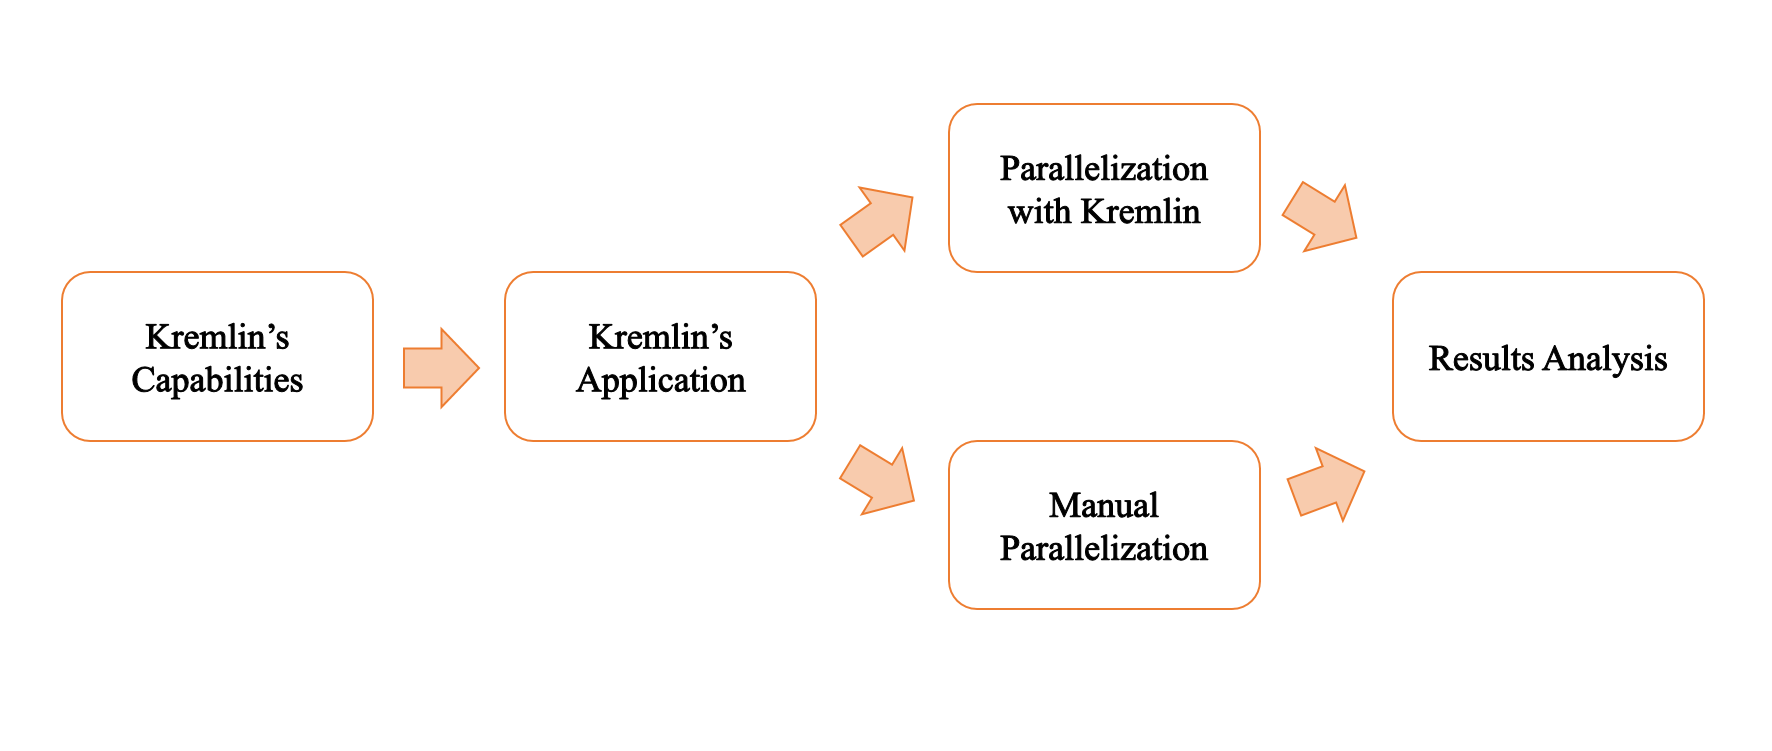
\includegraphics[width=1\textwidth]{methodology}
		\caption{Followed up methodology}
		\label{fig:method}
	\end{center}
\end{figure}


In the  figure ~\ref{fig:method} is outlined the steps that were followed to study the impact of the code being automatic parallelised. This methodology has five states. Firstly and using simple applications, an evaluation was made to Kremlin in order  to understand how to use this software tool and evaluate the results that Kremlin can achieve, for instance, if it has similar results comparing with an expert parallelizing manually the same code. After this, Kremlin will be applied to a set of codes with specific characteristics.

Before applying Kremlin, I manually parallelised the same sample of code in order to evaluate the results and, afterwards, compare with the Kremlin output. Since these states (the experiences with Kremlin and the manual code parallelization) required several attempts there were transitions between manual and Kremlin states. 

Finally, in the last state, after several attempts and tuning exercises applied to both code cases (manual and kremlin), data was collected from this experience to evaluate and validate its correctness in order to conclude how helpfull can automatic parallelization can be.

To sum up, this methodology as three main stages: learn and evaluate  Kremlin's uses and results; finding the tunning parameter through several attempts using Kremlin's outputs and manually parallelize the application's code; and, in the end, compare and analyze the results in every attempt to take conclusions; 


\subsection{Deep learn on Kremlin's usage}

Firstly, and according to all the presented tools/frameworks mentioned in the second chapter, \textit{Achieving the Highest Processing Power}, in the \textit{Using Code Parallelization} section ~\ref{sec:codeparallelization}, Kremlin was chosen because it presented the best results, easy usage and accessibility comparing to the other presented ones regarding the way the tool/framework could automatically parallelise code ~\ref{subsec:kremlin}.

Kremlin is a tool that indicates, for a serial program, which block can be parallelised and teorical calculated values, such as, overall speedup; self parallelism for each block; the ideal time reduced for each block, in percentage; the actual time reduced for each block, in percentage; and the block coverage considering the whole program, in percentage. The way this tool was used is as it follows: first, an object file, \textit{*.o} extension, is required from the compilation of a serial code. Afterwards, it is time to use the Kremlin's compiler with the generated object file so that it can profile the application. In order to do so, Kremlin's compiler runs the program as it is supposed to work. Now that the profiling is done, Kremlin generates the indications that should be followed to parallelise de provided serial code. It also includes the blocks that can be parallelised and the impact of this theoretical parallelization with the calculations done during the profiling. Since this parallelization report is done, the program has interpret it, confront with the code an apply it.

The Kremlin's usage seems easy, linear and fast forward, however it has some limitations that I experienced during the learning of Kremlin's capabilities: Kremlin's requires a specific environment mentioned in the Kremlin's repository ~\cite{KremlinRep}. It requires several software, libraries, compilers installations and a modern Unix operative system as its base, such as MAC OS, RHEL 7 or other Linux distribution compatible with the software specification required. Additionally, when installing the Kremlin's tool, some minor fixed are required in order to successfully install.

From the experiences that I have been through, Kremlin has another limitation: it can't compile and profile all kind of programs: it can only profile programs that use C/C++ as its programming language; programs that take advantage of data structures from the \textit{Standard Library}, such as, stack, list, priority queue, queue, list, hash table, map, multimap, heap, etc., since it doesn't recognize these structures; another Kremlin's limitations is its capability of compiling programs that have a deep function call level greater that seven. By deep function call level I mean the depth a function has starting from the \textit{main} function until it is called, like a tree function call tree. For instance: in a program there is the \textit{main()} function, a first level, that calls a \textit{foo1()} function, and this function calls a \textit{foo2()}, that this calls a \textit{foo3()} function, and so on. In this case, the deph of \textit{foo3()} function is four. Another small issue that kremlin's tool has is the definition of the iterator variable used in the \textit{for}'s loops must be defined outside of the loop, as it is in C programming language.


\subsection{Kremlin's application in specific code samples}

After all the experiences made in the previous state and as mentioned in the introduction of this chapter, the matrix multiplication algorithm was used to see the potentialities of Kremlin's compiler to profile and indicate the regions that can be parallelised. So, Kremlin was used in two similar, relatively in the code structure, matrix multiplication codes. The reason behind the choice was because these two versions of the algorithm are really close to one another, which means that the testing environment is similar to one another, consequently, the results should be similar. 

\subsection{Code parallelization with Kremlin's data}

Kremlin's tool just points the regions/blocks where the program can be parallelised. In both code samples there are various numbers of inner \textit{for} loops, for the \textit{Mult} code  there are three inner \textit{for} loops, which one of them has a degree of three and the rest a degree of two; and for the \textit{MultLine} code there are four inner \textit{for} loops, which one of them has a degree of three and the rest a degree of two aswell. At this time, after reading the report provided by Kremlin's tool, the developer must locate the loops, apply which loop should be parallelised, if it should be, and in case of inner \textit{for} loops, what loop should be parallelised using the OpenMP \textit{pragma} directives.

In my case, I followed all the instructions provided by Kremlin, located all the \textit{for} loops blocks indicated by kremlin's tool and applied the OpenMP \textit{pragma} directives. 

Following the two reports, ~\ref{code:onmulkremlinreport} ~\ref{code:onmulinekremlinreport}, and looking at the code's structure for both codes, it can be divided in 2 bigger parts: the \textit{for} loops used for matrices initialization and the \textit{for} loop for the matrix multiplication. With this information, code understanding and using an expert knowledge, the code parallelization was done.


\subsection{Manually Code parallelization}

In order to not be manipulated by the Kremlin's indications, the both codes were previously manually parallelised, this way it was guaranteed that the expert parallelization wasn't bias nor influenced.

For this parallelization, as mentioned before, it requires knowledge in, firstly, matrix multiplication algorithm; code understanding; best practice in what can and can't be parallelised, taking into account the overhead that could occur; and understand the thread behaviour in order to make it do the proper job without jeopardizing the programs outputs and/or possible caused overhead.  

Analysing the code, only the \textit{for} loop for the matrix multiplication was parallelised and applied the OpenMP \textit{pragma} directives applied to the innermost \textit{for} loop. In this case, each code as a slight difference because for the \textit{Mult} code each value of the result matrix but be calculated individually, so each thread is responsible for it and must treat that value as a private variable that isn't shared by the other threads. In the opposite, and since the \textit{MultLine} code calculates the values by adding the multiplication to the respective matrix's cell, each thread don't need to have their own private variable.

The bigger part of the code responsible for the matrices initialization wasn't parallelised, unlike in kremlin's case, because the gain would be noticeable on a large matrix size or it even could cause thread trampling, which could lead an overhead increase. 


\subsection{Results analysis}

To obtain the final execution time of each implementation (Original Matrix Multiplication ~\ref{code:onmul}, Original Matrix Multiplication by line ~\ref{code:onmuline}, Manual Matrix Multiplication by an expert ~\ref{code:onmulmanual}, Manual Matrix Multiplication by line by an expert ~\ref{code:onmulinemanual}, Kremlin Matrix Multiplication ~\ref{code:onmulkremlinreport} and Kremlin Matrix Multiplication by line~\ref{code:onmulinekremlin}), these six implementations suffered many modifications and tweaks since this process is a try-error until it is found the believed best parallelization. It is hardly possible to parallelise a whole program at the first try.

After compiling all these implementations and registering all the execution time for different matrix sizes and number of threads, in this case not applied to the original codes, this data was organized so it could be used to compare results and conclude about the performed experiences.

\section{Data collection from executed experiences}
-from kremlins' usage
-from kremlins output when using matrix multiplication
-times from original code
-Times from kremlins matrix multiplication
-times from maunally code parallelization
-variables: Pralellized vs not parallelized, matrix size, nº of threads)


In order to achieve such performance in the conditions mentioned in the problem's section, I purpose an autotuner or a concept proof that will enhance the application. For that, this autotuner will receive the program's original source code and though parallel optimization a new code will emerge. This code's modification will increase applications performance without jeopardizing the application's outcome.

\section{Data analysis method}
-3 versions of the same code (original, manual code parallelization, kremlins parallelization)
-Comparing execution time for each case
-Table and grafic analysis
-Impact for each concret case (increase or decrease in execution time)
To create this autotuner, the first step is to identify what parameters exist to tune and what impact they have in the application. For this matter, with the help of Kremlin and manual expert parallelization applications will increase its performance and parameters will be found. As Kremlin detect possible parallelized code and, additionally, measures the applications speedup with such modifications, and with manual expert parallelization, there will be a confront with these results and find what is better between these two scenarios. With this confrontation, and with different use cases, the tunning parameters will be found and the autotuner will be made.


\section{Data validation}
Comparing with teoric and expected results vs experimental results
To validate the whole methodology process, not only the autotuner itself but to compare the results between Kremlin outcomes and the code manually being parallelized, for evaluation metrics will be used: system energy consumptions when running the application; applications execution time; number of memory accesses and cache misses on the application; and the processing power measured by the number of instructions per secs. These evaluation metrics will be compared in three different cases: the original sequential code; manually paralleled code; and "automatic" paralleled code. In this last case it can be with Kremlin or with autotuner, depending in which of the methodology's state I am currently in.

To measure the above mentioned evaluation metrics, some libraries will be used: to measure energy consumptions RAPL will be used~\cite{Marcus}; to measure application  execution time OpemMP will be used ~\cite{Nc1998}; to measure number of memory accesses, cache misses and processing power PAPI ~\cite{Marcus} will be used.

Finally, two use cases will be used to validate this solution: a biopharmaceutical HPC application for accelerating drug discovery; and a self-adaptive navigation system to be used in smart cities. These use cases will be the applications that, the autotuner will try to achieve the highest processing power without jeopardizing the applications' outcome and having a low energy consumption.

\section{Experimental environment setup}

-Kremlins setup
-matrix mul setup
